\chapter{La cellule, unité du vivant}\label{ch:g6:cell-unit-of-life}

\Cref{ch:g5:first-look-at-cells} se terminait sur une promesse~: les
petites chambres ne sont pas vides. Cette année, le \omterm{def:g5:first-look-at-cells:microscope}{microscope} de
l'école ressort --- avec de meilleures lames et des questions plus
précises. Qu'y a-t-il exactement dans une \omterm{def:g5:first-look-at-cells:cell}{cellule}~? Les \omterm{def:g5:first-look-at-cells:cell}{cellules} de
\omterm{def:g1:plants-around-us:plant}{plantes} et d'\omterm{def:g1:animals-around-us:animal}{animaux} diffèrent-elles~? Et une \omterm{def:g5:first-look-at-cells:cell}{cellule} est-elle une
\emph{partie} du vivant, ou une seule \omterm{def:g5:first-look-at-cells:cell}{cellule} peut-elle être un \omterm{def:g6:exploring-our-environment:components}{être
vivant} entier~? La plus petite unité de la \omterm{def:g1:living-or-not:living}{biologie} mérite un
chapitre complet.

\section{À l'intérieur de la cellule}

\begin{definition}[Les parties de la cellule]\label{def:g6:cell-unit-of-life:parts}
Bien observée, toute \omterm{def:g5:first-look-at-cells:cell}{cellule} montre le même équipement de base~:
\begin{enumerate}
  \item la \emph{membrane}\index{membrane}, la fine enveloppe
        extérieure de la \omterm{def:g5:first-look-at-cells:cell}{cellule}, qui la tient d'un seul tenant et
        contrôle ce qui entre et ce qui sort~;
  \item le \emph{cytoplasme}\index{cytoplasme}, la gelée de
        remplissage où se fait le travail de la \omterm{def:g5:first-look-at-cells:cell}{cellule}~;
  \item le \emph{noyau}\index{noyau}
        (la tache sombre de
        \cref{rem:g5:first-look-at-cells:nucleus}), le centre de
        commande qui dirige la vie de la \omterm{def:g5:first-look-at-cells:cell}{cellule} et sa division.
\end{enumerate}
Membrane, cytoplasme, noyau~: le trousseau en trois pièces de
presque toutes les \omterm{def:g5:first-look-at-cells:cell}{cellules} de toutes les \omterm{def:g1:plants-around-us:plant}{plantes}, de tous les
\omterm{def:g1:animals-around-us:animal}{animaux} et de tous les \omterm{def:g6:decomposers-and-soil:decomposers}{champignons}.
\end{definition}

\begin{proposition}[Les cellules végétales ont des suppléments]\label{prop:g6:cell-unit-of-life:plantextras}
Les \omterm{def:g5:first-look-at-cells:cell}{cellules} végétales ajoutent leur propre équipement~:
\begin{itemize}
  \item une \emph{paroi}\index{paroi cellulaire} rigide à
        l'extérieur de la \omterm{def:g6:cell-unit-of-life:parts}{membrane} --- les parois qui font le
        briquetage de la pellicule d'oignon
        (\cref{ex:g5:first-look-at-cells:classics}) et donnent aux
        \omterm{def:g1:plants-around-us:plant}{plantes} leur tenue sans \omterm{def:g3:bones-and-muscles:skeleton}{os}~;
  \item des grains verts de la substance qui capte la \omterm{def:g6:exploring-our-environment:conditions}{lumière} dans
        le \omterm{def:g6:cell-unit-of-life:parts}{cytoplasme} --- les ateliers des \omterm{def:g5:food-webs:roles}{producteurs}
        (\cref{prop:g6:plants-are-producers:produce}), absents de
        toute \omterm{def:g5:first-look-at-cells:cell}{cellule} animale~;
  \item souvent une grande poche remplie d'eau dont la pression
        garde la \omterm{def:g5:first-look-at-cells:cell}{cellule} bien gonflée --- se faner
        (\cref{ex:g1:plants-around-us:wilt}), c'est le relâchement
        de ces poches.
\end{itemize}
\end{proposition}
\admitted

\begin{omfigure}
\begin{minipage}[t]{0.48\linewidth}\centering
\begin{tikzpicture}
  \node[anchor=south west, inner sep=0] (img) at (0,0)
    {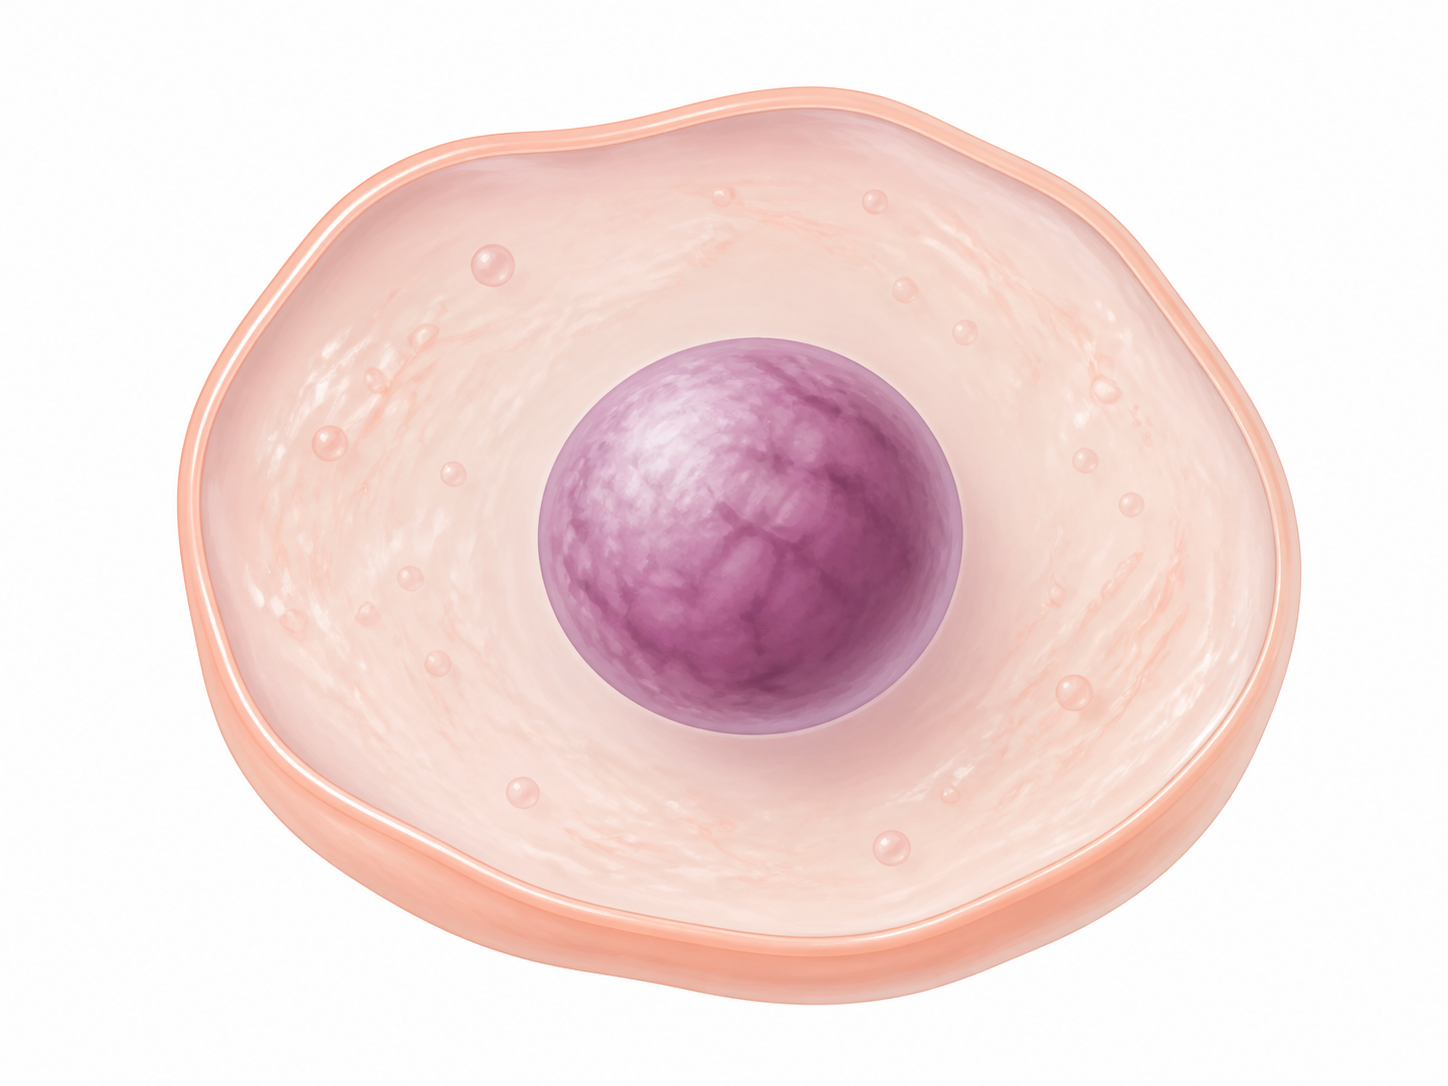
\includegraphics[width=0.9\linewidth]{images/book1/ai/fig-animal-cell.png}};
  \begin{scope}[x={(img.south east)}, y={(img.north west)},
      every node/.style={font=\footnotesize}]
    \draw[omDef, thick] (0.24,0.79) -- (0.12,0.93) node[above] {membrane};
    \draw[omDef, thick] (0.32,0.42) -- (0.15,0.20)
      node[below] {cytoplasme};
    \draw[omDef, thick] (0.58,0.52) -- (0.80,0.20)
      node[below] {noyau};
  \end{scope}
\end{tikzpicture}

{\small \omterm{def:g5:first-look-at-cells:cell}{cellule} animale~:\\ \omterm{def:g6:cell-unit-of-life:parts}{membrane}, \omterm{def:g6:cell-unit-of-life:parts}{cytoplasme}, \omterm{def:g6:cell-unit-of-life:parts}{noyau}}
\end{minipage}\hfill
\begin{minipage}[t]{0.48\linewidth}\centering
\begin{tikzpicture}
  \node[anchor=south west, inner sep=0] (img) at (0,0)
    {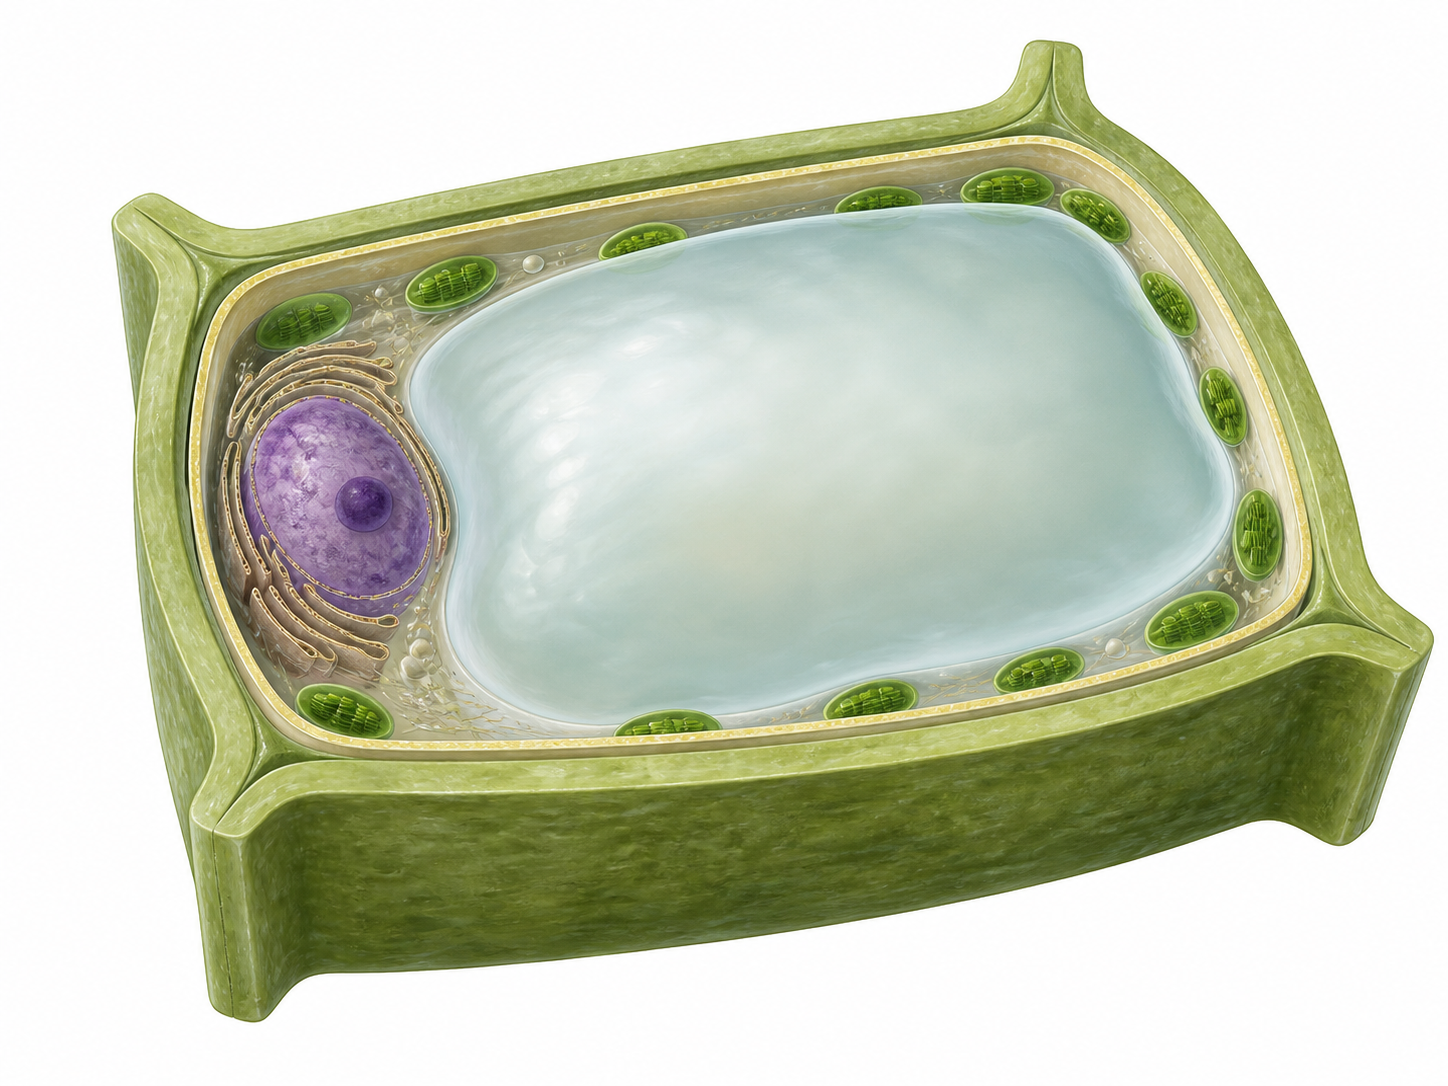
\includegraphics[width=0.98\linewidth]{images/book1/ai/fig-plant-cell.png}};
  \begin{scope}[x={(img.south east)}, y={(img.north west)},
      every node/.style={font=\footnotesize}]
    \draw[omMeth!60!black, thick] (0.16,0.80) -- (0.08,0.94)
      node[above] {paroi};
    \draw[omDef, thick] (0.26,0.53) -- (0.22,-0.04)
      node[below] {noyau};
    \draw[omMeth!60!black, thick] (0.72,0.24) -- (0.85,-0.04)
      node[below] {grains verts};
    \draw[omDef!70, thick] (0.62,0.55) -- (0.70,1.04)
      node[above] {poche d'eau};
  \end{scope}
\end{tikzpicture}

{\small \omterm{def:g5:first-look-at-cells:cell}{cellule} végétale~: le même trousseau, plus la paroi,\\ les
grains verts et la poche d'eau}
\end{minipage}

\medskip
{\small Les deux \omterm{def:g5:first-look-at-cells:cell}{cellules} classiques \omterm{def:g3:bones-and-muscles:skeleton}{côte} à \omterm{def:g3:bones-and-muscles:skeleton}{côte}. Le même trousseau
en trois pièces~; la \omterm{def:g5:first-look-at-cells:cell}{cellule} végétale y ajoute sa paroi, ses grains
verts et sa poche d'eau bien gonflée.}
\end{omfigure}

\begin{example}[Distinguer les lames]\label{ex:g6:cell-unit-of-life:slides}
De retour au \omterm{def:g5:first-look-at-cells:microscope}{microscope} avec les deux lames de
\cref{ex:g5:first-look-at-cells:classics}, les différences ont
maintenant un nom. Pellicule d'oignon~: des parois droites qui se
rejoignent en angles --- les \omterm{prop:g6:cell-unit-of-life:plantextras}{parois cellulaires}~; un \omterm{def:g6:cell-unit-of-life:parts}{noyau} repoussé
sur le côté --- l'ouvrage de la poche d'eau. \omterm{def:g5:first-look-at-cells:cell}{Cellules} de joue~: pas
de parois, des contours souples et arrondis --- la \omterm{def:g6:cell-unit-of-life:parts}{membrane} seule
--- le \omterm{def:g6:cell-unit-of-life:parts}{noyau} vers le milieu. Un coup d'\omterm{def:g1:the-five-senses:sense}{œil} suffit maintenant à lire
végétal ou \omterm{def:g1:animals-around-us:animal}{animal}.
\end{example}

\section{Des vies entières dans une seule cellule}

\begin{definition}[Êtres vivants unicellulaires]\label{def:g6:cell-unit-of-life:unicellular}
Un \omterm{def:g6:exploring-our-environment:components}{être vivant} \emph{unicellulaire}\index{unicellulaire} est un
organisme complet fait d'exactement une \omterm{def:g5:first-look-at-cells:cell}{cellule}
(\cref{rem:g5:first-look-at-cells:onecelled}). Dans une seule
\omterm{def:g6:cell-unit-of-life:parts}{membrane}, il se nourrit, se déplace, perçoit et se reproduit --- en
se divisant en deux (la division de
\cref{prop:g5:first-look-at-cells:growth}, comme histoire d'une vie
entière). La \omterm{ex:g6:producing-our-food:bread}{levure} de
\cref{ex:g6:producing-our-food:bread} en est un~; les nageurs de
n'importe quelle goutte de mare aussi, ainsi que la plupart des
\omterm{def:g6:producing-our-food:fermentation}{microbes} du \omterm{def:g6:decomposers-and-soil:soil}{sol}, du yaourt et des mains.
\end{definition}

\begin{example}[Une goutte d'eau de mare, visitée]\label{ex:g6:cell-unit-of-life:drop}
Une goutte prélevée sur la paroi verte de l'aquarium, sous
l'objectif~: une \omterm{def:g5:first-look-at-cells:cell}{cellule} en forme de pantoufle qui rame en battant
de ses cils, plus vite que tout le reste du champ~; des \omterm{def:g5:first-look-at-cells:cell}{cellules}
uniques et vertes --- des \omterm{def:g5:food-webs:roles}{producteurs} nageurs, qui captent la
\omterm{def:g6:exploring-our-environment:conditions}{lumière} comme n'importe quelle \omterm{def:g1:plants-around-us:parts}{feuille}~; une masse qui coule autour
de sa nourriture et l'avale tout entière. Chacune se nourrit, se
déplace, esquive --- toute la vie d'un \omterm{def:g1:animals-around-us:animal}{animal} ou d'une \omterm{def:g1:plants-around-us:plant}{plante}, tenue
dans le budget d'une seule \omterm{def:g5:first-look-at-cells:cell}{cellule}.
\end{example}

\begin{remark}[Une cellule ou beaucoup~: deux façons d'être vivant]\label{rem:g6:cell-unit-of-life:twoways}
Un organisme \omterm{def:g6:cell-unit-of-life:unicellular}{unicellulaire} fait tout avec une seule \omterm{def:g5:first-look-at-cells:cell}{cellule}~; ton
corps fait tout avec des dizaines de milliers de milliards de
\omterm{def:g5:first-look-at-cells:cell}{cellules} \emph{spécialisées} --- des \omterm{def:g5:first-look-at-cells:cell}{cellules} de joue pour tapisser,
des \omterm{def:g5:first-look-at-cells:cell}{cellules} musculaires qui se contractent
(\cref{def:g3:bones-and-muscles:muscle}), des \omterm{def:g5:first-look-at-cells:cell}{cellules} nerveuses qui
portent les messages de \cref{prop:g5:brain-in-command:loop}.
Beaucoup de \omterm{def:g5:first-look-at-cells:cell}{cellules} permettent la division du travail~; une seule
\omterm{def:g5:first-look-at-cells:cell}{cellule} veut dire tous les métiers dans une seule pièce. Les deux
plans fonctionnent~: les \omterm{def:g6:cell-unit-of-life:unicellular}{unicellulaires} sont les \omterm{def:g6:exploring-our-environment:components}{êtres vivants} les
plus nombreux de la Terre.
\end{remark}

\section{La théorie cellulaire}

\begin{proposition}[La théorie cellulaire]\label{prop:g6:cell-unit-of-life:theory}
Deux phrases, mûries pendant des siècles, résument ce chapitre et
\cref{ch:g5:first-look-at-cells}~:
\begin{enumerate}
  \item tout \omterm{def:g6:exploring-our-environment:components}{être vivant} est fait d'une ou de plusieurs \omterm{def:g5:first-look-at-cells:cell}{cellules},
        les plus petites \omterm{prop:g5:first-look-at-cells:principle}{unités du vivant}~;
  \item toute \omterm{def:g5:first-look-at-cells:cell}{cellule} provient de la division d'une \omterm{def:g5:first-look-at-cells:cell}{cellule}
        existante.
\end{enumerate}
Aucune exception n'a jamais été trouvée --- ni dans les mers les
plus profondes, ni dans la plus ancienne flaque de rocher. La
seconde phrase a une conséquence considérable~: toute \omterm{def:g5:first-look-at-cells:cell}{cellule}
vivante aujourd'hui prolonge une chaîne ininterrompue de divisions
qui remonte aux premiers vivants --- la \omterm{prop:g6:classification-kinship:kinship}{parenté}
(\cref{prop:g6:classification-kinship:kinship}) écrite à l'échelle
de la \omterm{def:g5:first-look-at-cells:cell}{cellule}.
\end{proposition}
\admitted

\begin{method}[Lire n'importe quel organisme à l'échelle cellulaire]\label{met:g6:cell-unit-of-life:read}
Devant n'importe quel \omterm{def:g6:exploring-our-environment:components}{être vivant}~:
\begin{enumerate}
  \item demande-toi d'abord~: une \omterm{def:g5:first-look-at-cells:cell}{cellule}, ou beaucoup~?
  \item si beaucoup~: attends-toi à des sortes spécialisées ---
        pour tapisser, transporter, contracter, commander~;
  \item végétal ou \omterm{def:g1:animals-around-us:animal}{animal}~? cherche des parois et des grains verts
        au \omterm{def:g5:first-look-at-cells:microscope}{microscope}~;
  \item toute croissance, réparation ou reproduction que tu
        observes~: traduis-la en divisions de \omterm{def:g5:first-look-at-cells:cell}{cellules} --- la
        phrase 2 garantit que la traduction existe.
\end{enumerate}
\end{method}

\begin{example}[La théorie à l'œuvre dans ce livre]\label{ex:g6:cell-unit-of-life:atwork}
La phrase 1 fondait l'\omterm{prop:g5:first-look-at-cells:principle}{unité du vivant}
(\cref{prop:g5:first-look-at-cells:principle})~; la phrase 2 fondait
la croissance par division
(\cref{ex:g5:first-look-at-cells:one}), la \omterm{ex:g6:producing-our-food:bread}{levure} qui double dans la
pâte, les \omterm{def:g6:decomposers-and-soil:decomposers}{décomposeurs} qui se multiplient dans le tas tiède, et les
main-d'œuvres de \omterm{def:g6:producing-our-food:fermentation}{microbes} de
\cref{ch:g6:producing-our-food}. Une petite théorie, qui porte une
grande part de la \omterm{def:g1:living-or-not:living}{biologie} de cette année.
\end{example}

\section{Exercices}

\begin{exercise}[$\star$]\label{exo:g6:cell-unit-of-life:1}
Nomme le trousseau en trois pièces de toute \omterm{def:g5:first-look-at-cells:cell}{cellule}, avec le travail
de chaque pièce.
\end{exercise}

\begin{exercise}[$\star$]\label{exo:g6:cell-unit-of-life:2}
Nomme les trois suppléments de la \omterm{def:g5:first-look-at-cells:cell}{cellule} végétale et ce que fait
chacun.
\end{exercise}

\begin{exercise}[$\star$]\label{exo:g6:cell-unit-of-life:3}
Au \omterm{def:g5:first-look-at-cells:microscope}{microscope}, comment distingues-tu une \omterm{def:g5:first-look-at-cells:cell}{cellule} de pellicule
d'oignon d'une \omterm{def:g5:first-look-at-cells:cell}{cellule} de joue~? Deux différences visibles.
\end{exercise}

\begin{exercise}[$\star$]\label{exo:g6:cell-unit-of-life:4}
Qu'est-ce qu'un \omterm{def:g6:exploring-our-environment:components}{être vivant} \omterm{def:g6:cell-unit-of-life:unicellular}{unicellulaire}~? Nommes-en deux tirés de
ce chapitre.
\end{exercise}

\begin{exercise}[$\star$]\label{exo:g6:cell-unit-of-life:5}
Énonce les deux phrases de la théorie cellulaire.
\end{exercise}

\begin{exercise}[$\star$]\label{exo:g6:cell-unit-of-life:6}
Comment un organisme \omterm{def:g6:cell-unit-of-life:unicellular}{unicellulaire} se reproduit-il~?
\end{exercise}

\begin{exercise}[$\star\star$]\label{exo:g6:cell-unit-of-life:7}
Pourquoi les \omterm{def:g1:plants-around-us:plant}{plantes} tiennent-elles debout sans \omterm{def:g3:bones-and-muscles:skeleton}{os}~? Quelles deux
pièces de l'équipement de la \omterm{def:g5:first-look-at-cells:cell}{cellule} végétale se partagent ce
travail --- et qu'est-ce que se faner, à l'échelle de la \omterm{def:g5:first-look-at-cells:cell}{cellule}~?
\end{exercise}

\begin{exercise}[$\star\star$]\label{exo:g6:cell-unit-of-life:8}
Quelle partie de la \omterm{def:g5:first-look-at-cells:cell}{cellule} est l'atelier des \omterm{def:g5:food-webs:roles}{producteurs} de
\cref{prop:g6:plants-are-producers:produce}~? Pourquoi toute \omterm{def:g5:first-look-at-cells:cell}{cellule}
animale doit-elle en être dépourvue, d'après
\cref{prop:g6:matter-from-food:transform}~?
\end{exercise}

\begin{exercise}[$\star\star$]\label{exo:g6:cell-unit-of-life:9}
Donne trois sortes de \omterm{def:g5:first-look-at-cells:cell}{cellules} spécialisées de ton corps et le
métier de chacune, d'après \cref{rem:g6:cell-unit-of-life:twoways}.
\end{exercise}

\begin{exercise}[$\star\star$]\label{exo:g6:cell-unit-of-life:10}
Traduis en divisions de \omterm{def:g5:first-look-at-cells:cell}{cellules}, selon
\cref{met:g6:cell-unit-of-life:read}~: une éraflure qui guérit~; une
pâte qui double dans la nuit~; un têtard qui grandit.
\end{exercise}

\begin{exercise}[$\star\star$]\label{exo:g6:cell-unit-of-life:11}
Les nageurs verts de la goutte de mare sont des \omterm{def:g5:first-look-at-cells:cell}{cellules} uniques qui
captent la \omterm{def:g6:exploring-our-environment:conditions}{lumière}. Quel métier de
\cref{def:g5:food-webs:roles} exercent-ils, et qu'est-ce que cela
fait d'eux dans le \omterm{def:g5:food-webs:web}{réseau alimentaire} de la mare~?
\end{exercise}

\begin{exercise}[$\star\star\star$]\label{exo:g6:cell-unit-of-life:12}
Prends au sérieux la seconde phrase de la théorie cellulaire, comme
\cref{rem:g6:classification-kinship:implies} prenait l'arbre~:
quelle chaîne ininterrompue relie l'une de tes \omterm{def:g5:first-look-at-cells:cell}{cellules} de joue au
passé lointain~? Énonce la conséquence en une phrase.
\end{exercise}

\section{Problème~: l'après-midi de microscopie}

\begin{problem}[{Problème du week-end --- quatre lames, une
théorie}]\label{pb:g6:cell-unit-of-life:1}
L'après-midi de microscopie de la classe~: quatre postes, quatre
lames --- pellicule d'oignon (A), grattage de joue (B), une goutte
d'eau de mare (C), un frottis de yaourt (D). Chaque équipe fait le
tour des quatre et tient ses dessins.

\medskip\noindent\textbf{Partie I --- Les postes A et B.}
\begin{enumerate}
  \item Au poste A, l'équipe dessine des «~briques~» à parois
        droites, chacune avec une tache sombre serrée d'un côté.
        Nomme la paroi, la tache, et le coupable de ce
        tassement.
  \item Au poste B~: des \omterm{def:g5:first-look-at-cells:cell}{cellules} arrondies, sans parois, avec des
        taches centrales. Énumère l'équipement que les \omterm{def:g5:first-look-at-cells:cell}{cellules} de
        A possèdent et que celles de B n'ont pas --- et le
        trousseau que les deux partagent.
  \item Un camarade demande pourquoi les \omterm{def:g5:first-look-at-cells:cell}{cellules} d'oignon, venues
        d'un \omterm{ex:g4:plants-without-seeds:bulbtuber}{bulbe} poussé sous terre, ne montrent aucun grain vert.
        Réponds avec le travail des grains et l'adresse du \omterm{ex:g4:plants-without-seeds:bulbtuber}{bulbe}.
  \item À qui sont les \omterm{def:g5:first-look-at-cells:cell}{cellules} de la lame B~? Dis ce que cela
        implique par la phrase 2 de la théorie cellulaire~: d'où
        vient chacune de ces \omterm{def:g5:first-look-at-cells:cell}{cellules}~?
\end{enumerate}

\medskip\noindent\textbf{Partie II --- Les postes C et D.}
\begin{enumerate}[resume]
  \item Poste C~: la rameuse en forme de pantoufle, les nageurs
        verts, la masse qui coule. Pour chacun, nomme les
        activités vitales visibles en une minute d'observation ---
        et conclus ce qu'est chacun.
  \item Les nageurs verts sont des \omterm{def:g5:first-look-at-cells:cell}{cellules} uniques et pourtant des
        \omterm{def:g5:food-webs:roles}{producteurs}. Quelle pièce d'équipement le dessin doit-il
        montrer pour le prouver~?
  \item Le frottis de yaourt du poste D montre de minuscules
        \omterm{def:g5:first-look-at-cells:cell}{cellules} par paires et en chaînes, en très grand nombre.
        Relie-les à \cref{ex:g6:producing-our-food:yogurt}~: qu'ont
        fait ces \omterm{def:g5:first-look-at-cells:cell}{cellules} au \omterm{def:g2:animals-grow-up:born}{lait}, et que sont-elles, dans le
        vocabulaire de ce chapitre~?
  \item Une équipe affirme que la lame D ne montre «~aucun \omterm{def:g6:exploring-our-environment:components}{être
        vivant}, juste des grains~». Quelle observation unique ---
        avec de la patience ou une lame tiédie --- trancherait la
        question de savoir si ces grains vivent, d'après la phrase
        2 de la théorie cellulaire~?
\end{enumerate}

\medskip\noindent\textbf{Partie III --- La rédaction.}
\begin{enumerate}[resume]
  \item Le compte rendu doit ranger les quatre lames selon~: une
        \omterm{def:g5:first-look-at-cells:cell}{cellule} ou beaucoup~? végétal, \omterm{def:g1:animals-around-us:animal}{animal} ou ni l'un ni
        l'autre~? Fais-le.
  \item Chaque dessin de l'après-midi montre le même trousseau en
        trois pièces. Énonce ce trousseau, et dis de quoi son
        universalité est la preuve
        (\cref{prop:g5:first-look-at-cells:principle}).
  \item L'enseignante conclut~: «~tout ce que vous avez dessiné
        aujourd'hui a un jour été une seule \omterm{def:g5:first-look-at-cells:cell}{cellule}~». Défends la
        phrase pour l'oignon, pour la propriétaire des \omterm{def:g5:first-look-at-cells:cell}{cellules} de
        joue et pour les chaînes du yaourt.
  \item Formule la découverte de l'après-midi sous forme de théorie
        cellulaire --- deux phrases --- et indique, pour chaque
        lame, quelle phrase elle a le mieux illustrée.
\end{enumerate}
\end{problem}
